\documentclass[11pt,a4paper]{article}
\usepackage[margin=24mm]{geometry}\usepackage{fontspec,unicode-math,booktabs,graphicx,hyperref}\setmainfont{STIXGeneral}\setmathfont{STIX Two Math}\hypersetup{hidelinks}
\title{A complete-manuscript comparison for diagonal twistings}\author{Human Compression Project}\date{11 October 2026}
\begin{document}\maketitle
The original is Piedade and Tranchida's \emph{Coset geometries acting on their elements: The $j$-diagonals twisting}, arXiv:2608.23223v1 (N007, twelve pages). The replacement comprises the entire common paper \emph{Orbit intersections and regular semidirect geometries} and the entire application \emph{Diagonal twistings and finite tree diagrams}, five pages each. Both use the published, independently reviewed quotient repair. One original is compared, not the thirty-two detailed scientific clauses. N006 is background and receives no whole-original credit here.

\paragraph{The whole topic and the conditional application.}
Let $L$ be the whole source, $U$ the whole common paper, $A$ the complete application and $P$ the complete validation program. The primary coordinate is calibrated selected NFC characters excluding whitespace:
\begin{center}\begin{tabular}{lrr}\toprule
Complete document & Pages & Characters\\\midrule
Original N007 & 12 & 22,888\\
Common theory & 5 & 10,968\\
Application & 5 & 11,771\\
Full validation appendix & 2 & 3,161\\\bottomrule
\end{tabular}\end{center}
All front matter, references, author information, source diagrams' extracted text and the version stamp remain. Only exact repeated furniture and physical page numbers are removed. The common paper is fully charged to this topic regardless of overlaps with any other topic.
\[
 R_{\rm written}=\frac{c(L)}{c(U)+c(A)}=1.007,\qquad
 r\mid(U,P)=\frac{c(L)}{c(A)}=1.944.
\]
The conditional comparison assumes that \emph{the full common paper and the whole declared program have already been acquired}. It is not a whole-topic saving. In the primary coordinate the written replacement is only slightly shorter; including the full validation software makes it longer:
\begin{center}\begin{tabular}{lr}\toprule
Complete denominator & Source/denominator\\\midrule
Written papers & 1.007\\
Written papers plus full printed program & 0.884\\
Written papers plus full raw program & 0.894\\\bottomrule
\end{tabular}\end{center}
The raw validation program costs 2,856 nonspace characters. Printed and raw programs are alternatives, never added together. Zero uniform mathematical claims rely on these finite samples. The two operational drivers (6,059 and 2,541) and Lean source (2,587) are separate inventories. Eight scoped declarations do not provide a complete formalization. A factor below one means a longer replacement in that coordinate.
\newpage
\begin{center}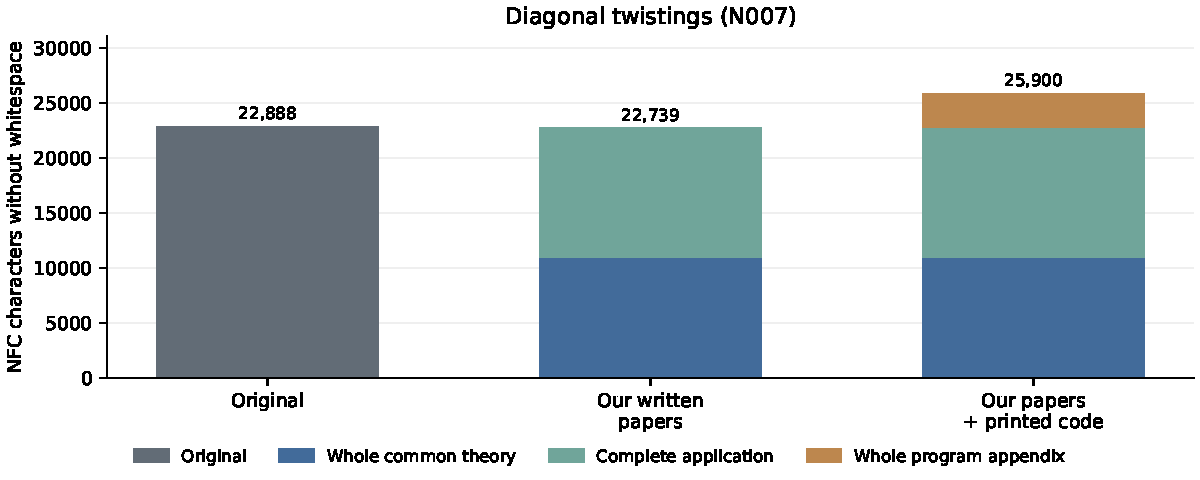
\includegraphics[width=\textwidth]{whole_costs.pdf}\end{center}
The stacks charge every common and application page, then the entire printed validation program where shown. One application cannot establish a repeated sawtooth pattern or a minimum proof complexity.

\paragraph{Unit and representation sensitivity.}
The following uses calibrated selected text under NFC:
\begin{center}\begin{tabular}{lrrr}\toprule
Unit & Whole written & Conditional & With printed program\\\midrule
Whitespace tokens & 0.898 & 1.740 & 0.849 \\
Alphanumeric runs & 1.035 & 1.993 & 0.915 \\
Nonspace characters & 1.007 & 1.944 & 0.884 \\
Collapsed-space characters & 0.988 & 1.909 & 0.878 \\
Collapsed-space UTF-8 bytes & 0.923 & 1.813 & 0.831 \\
\bottomrule\end{tabular}\end{center}
The exact data retain all five units under NFC and NFKC in three variants: raw untrimmed, raw selected and calibrated selected. They give thirty coordinates and 120 fractions. Raw untrimmed counts preserve page furniture on both sides. The written replacement is longer in whitespace tokens, collapsed-space characters and UTF-8 bytes. These are representation-sensitive lengths; a near-unit primary factor is not evidence of a unit-independent reduction or of deep mathematical compression.

\paragraph{Scope, attribution and costs not measured.}
The accepted contract recovers both diagonal constructions and their full parabolics, exact doubled labels including infinity, invariant quotients under the stated hypertope hypothesis, finite trees with at most one exceptional edge label, and the named classical polytope comparisons. Arbitrary finite diagrams remain an open question in this source contract. The corrected argument uses intersections of maximal-parabolic images in quotient geometries; it does not assert that every quotient is a hypertope. Classical Coxeter embeddings, the polytope correspondence and the named constructions retain their stated outside hypotheses and attributions.

The distinct input audit accepted every complete page, 120 PDF and forty raw-file cells. Seven visible delimiter components whose font encoding produces whitespace were retained, while generated line breaks remained whitespace. The duplicated Form callback affects metadata only: the version stamp stays once in returned text. Seventeen classes checked against actual outlines supply 237 substitutions. Directional diagram strokes are separate visible components, not a full encoding of the graphs.

Full graphics, retained external proofs, unavailable historical software and a complete formalization have unknown cost, not zero. This packet changes no scientific or conjecture credit and leaves every earlier numerical report immutable. Its arithmetic, actual plotted bars and reader require distinct review before these factors are admitted.
\end{document}
